\documentclass{standalone}
\usepackage{amsmath}
\usepackage{tikz}

\begin{document}
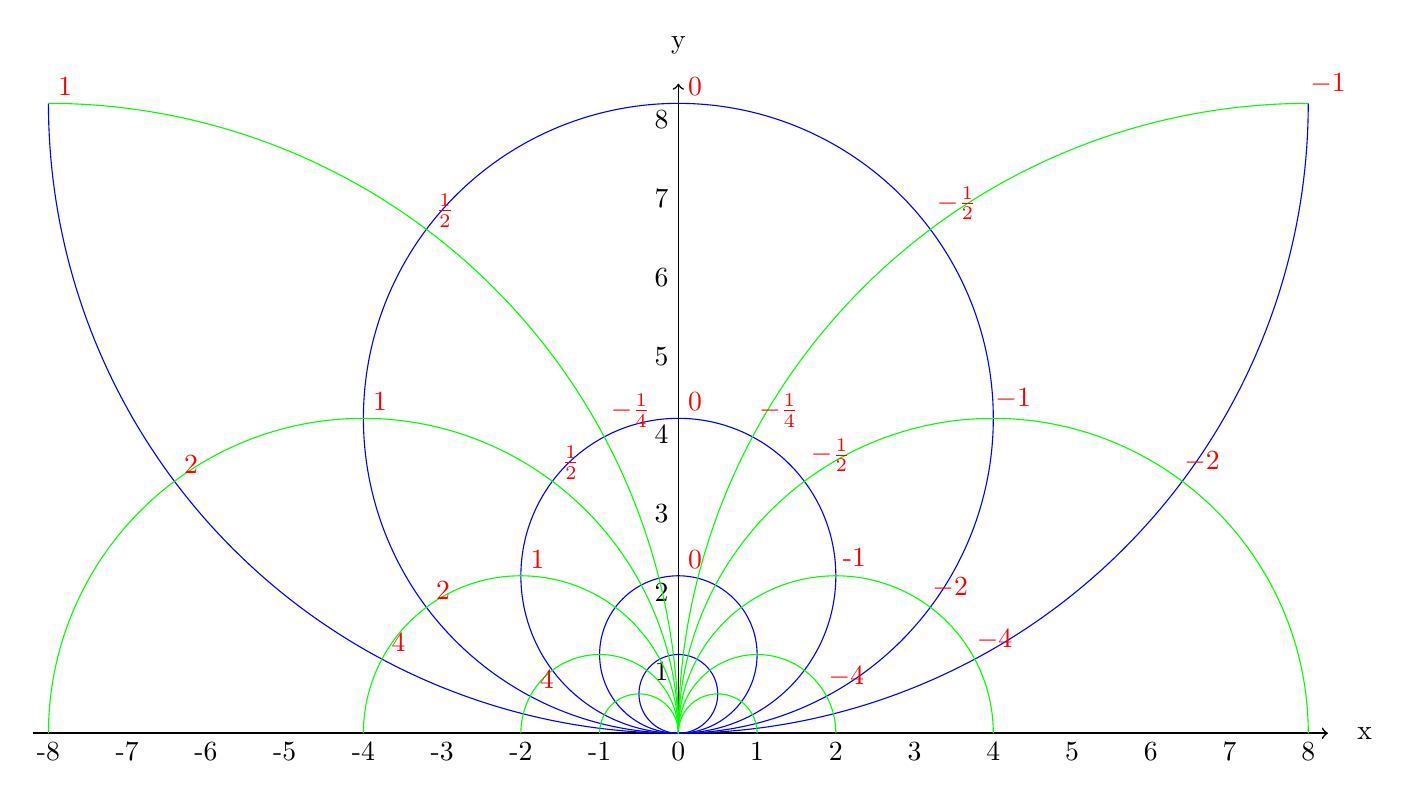
\begin{tikzpicture}
\draw [black, line width=0.6pt, ->] (0,0) to[out=90,in=270] (0,8.25);
\node [anchor=south] at (0,8.5) {y};
\draw [black, line width=0.6pt, ->] (-8.2,0) to[out=0,in=180] (8.25,0);
\node [anchor=west] at (8.5,0) {x};
\foreach \x in {-8,-7,-6,-5,-4,-3,-2,-1,0,1,2,3,4,5,6,7,8}
  \node [anchor=north] at (\x,0) {\x};
\foreach \y in {1,2,3,4,5,6,7,8}
  \node [anchor=45] at (0,\y) {\y};

\begin{scope}
  \draw[blue,scale=1.0,samples=360,domain=0.0:360,variable=\t] plot ({0.5 * cos(\t) },{0.5 + 0.5 * sin(\t)});
  \draw[blue,scale=1.0,samples=360,domain=0.0:360,variable=\t] plot ({1 * cos(\t) },{1 + 1 * sin(\t)});
  \draw[blue,scale=1.0,samples=360,domain=0.0:360,variable=\t] plot ({2 * cos(\t) },{2 + 2 * sin(\t)});
  \draw[blue,scale=1.0,samples=360,domain=0.0:360,variable=\t] plot ({4 * cos(\t) },{4 + 4 * sin(\t)});
  \draw[blue,scale=1.0,samples=360,domain=-180:0.0,variable=\t] plot ({8 * cos(\t) },{8 + 8 * sin(\t)});

  \draw[green,scale=1.0,samples=360,domain=0.0:180,variable=\t] plot ({0.5 + 0.5 * cos(\t) },{0.5 * sin(\t)});
  \draw[green,scale=1.0,samples=360,domain=0.0:180,variable=\t] plot ({1 + 1 * cos(\t) },{1 * sin(\t)});
  \draw[green,scale=1.0,samples=360,domain=0.0:180,variable=\t] plot ({2 + 2 * cos(\t) },{2 * sin(\t)});
  \draw[green,scale=1.0,samples=360,domain=0.0:180,variable=\t] plot ({4 + 4 * cos(\t) },{4 * sin(\t)});
  \draw[green,scale=1.0,samples=360,domain=90:180,variable=\t] plot ({8 + 8 * cos(\t) },{8 * sin(\t)});

  \draw[green,scale=1.0,samples=360,domain=0.0:180,variable=\t] plot ({-0.5 + 0.5 * cos(\t) },{0.5 * sin(\t)});
  \draw[green,scale=1.0,samples=360,domain=0.0:180,variable=\t] plot ({-1 + 1 * cos(\t) },{1 * sin(\t)});
  \draw[green,scale=1.0,samples=360,domain=0.0:180,variable=\t] plot ({-2 + 2 * cos(\t) },{2 * sin(\t)});
  \draw[green,scale=1.0,samples=360,domain=0.0:180,variable=\t] plot ({-4 + 4 * cos(\t) },{4 * sin(\t)});
  \draw[green,scale=1.0,samples=360,domain=0.0:90.0,variable=\t] plot ({-8 + 8 * cos(\t) },{8 * sin(\t)});

  \node [anchor=225, red] at (64/17, 16/17) {$-4$};
  \node [anchor=225, red] at (32/5, 16/5) {$-2$};
  \node [anchor=225, red] at (8, 8) {$-1$};
  \node [anchor=225, red] at (-8, 8) {$1$};
  \node [anchor=225, red] at (-32/5, 16/5) {$2$};
  \node [anchor=225, red] at (-64/17, 16/17) {$4$};

  \node [anchor=225, red] at (32/17, 8/17) {$-4$};
  \node [anchor=225, red] at (16/5, 8/5) {$-2$};
  \node [anchor=225, red] at (4, 4) {$-1$};
  \node [anchor=225, red] at (16/5, 32/5) {$-\frac{1}{2}$};
  \node [anchor=225, red] at (0, 8) {$0$};
  \node [anchor=225, red] at (-16/5, 32/5) {$\frac{1}{2}$};
  \node [anchor=225, red] at (-4, 4) {$1$};
  \node [anchor=225, red] at (-16/5, 8/5) {$2$};
  \node [anchor=225, red] at (-32/17, 8/17) {$4$};

  \node [anchor=225, red] at (2, 2) {-1};
  \node [anchor=225, red] at (8/5, 16/5) {$-\frac{1}{2}$};
  \node [anchor=225, red] at (16/17, 64/17) {$-\frac{1}{4}$};
  \node [anchor=225, red] at (0, 4) {$0$};
  \node [anchor=225, red] at (-16/17, 64/17) {$-\frac{1}{4}$};
  \node [anchor=225, red] at (-8/5, 16/5) {$\frac{1}{2}$};
  \node [anchor=225, red] at (-2, 2) {1};

  \node [anchor=225, red] at (0, 2) {$0$};

\end{scope}

\end{tikzpicture}
\end{document}
